\documentclass{beamer}
\usepackage[english,russian]{babel}
\usepackage[utf8]{inputenc}
\usepackage{amsmath}
\usepackage{hyperref}
\usetheme{Warsaw}
\usepackage{listings}
\usepackage{xcolor}
\usepackage{tikz}
\usetikzlibrary{graphs}
\usepackage{algpseudocode}

\lstset{
    frame=tb,
    tabsize=4,
    showstringspaces=false,
    numbers=left,
    commentstyle=\color{green},
    keywordstyle=\color{blue},
    stringstyle=\color{red},
    emph={baz},
    emphstyle=\textbf
}

\begin{document}

\title{Задачи разрешимости логических формул и приложения\newline Лекция 6. Линейная логика. Логика битовых векторов}
\author{Роман Холин}
\institute{Московский государственный университет}
\date{Москва, 2022}

\begin{frame}
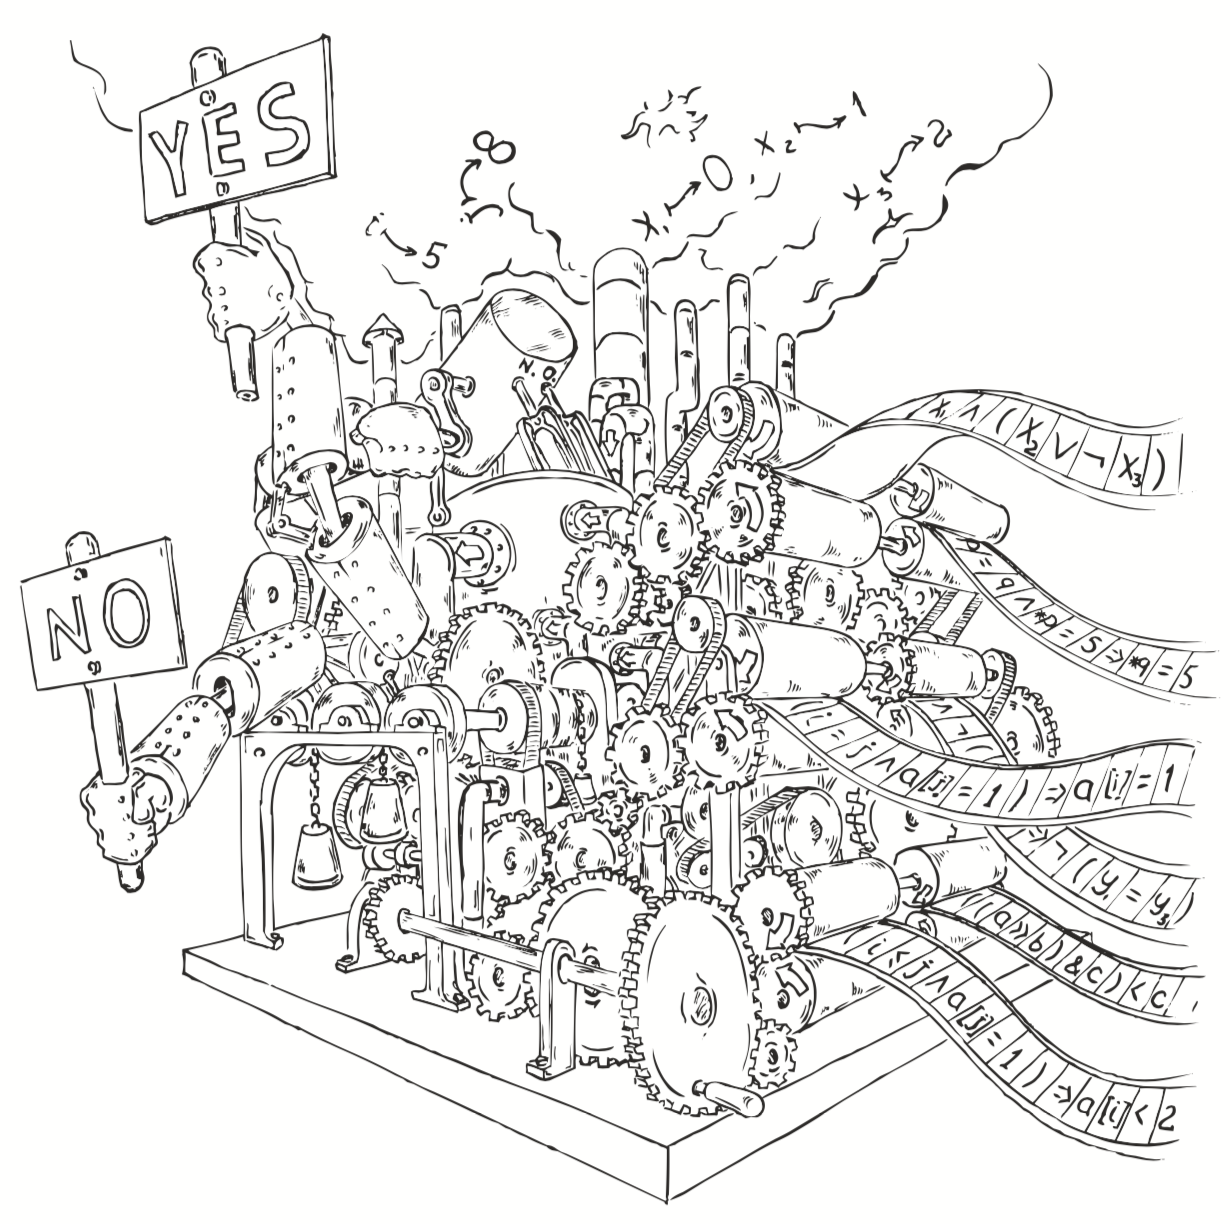
\includegraphics[scale=0.5]{../decision-procedure.png}
\end{frame}

\frame{\titlepage}

\begin{frame}{Логика линейной арифметики}
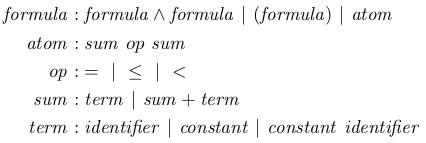
\includegraphics[scale=0.5]{linear_syntax.png}
\end{frame}

\begin{frame}{Логика линейной арифметики}
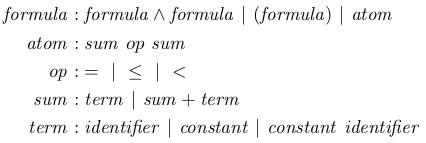
\includegraphics[scale=0.5]{linear_syntax.png}
$2z_1 + 3z_2 \le 5 \wedge z_2 + 5z_2 - 10z_3 \ge 6 \wedge z1 + z3 = 3$
\end{frame}

\begin{frame}{Домен}
\begin{itemize}
\item Целые числа
\item Рациональные числа
\end{itemize}
\end{frame}

\begin{frame}{Домен}
\begin{itemize}
\item Целые числа - целочисленное линейное программирование
\item Рациональные числа - симлекс метод
\end{itemize}
\end{frame}

\begin{frame}{Логика битовых векторов}
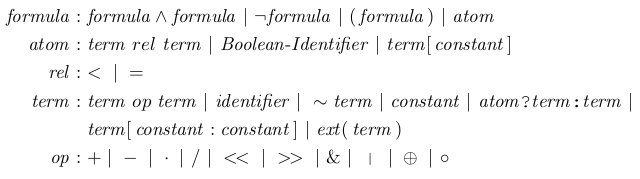
\includegraphics[scale=0.5]{bit_syntax.png}
\end{frame}

\begin{frame}{Мотивация}
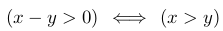
\includegraphics[scale=0.5]{mot1.png}
\end{frame}

\begin{frame}{Мотивация}
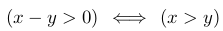
\includegraphics[scale=0.5]{mot1.png}\newline
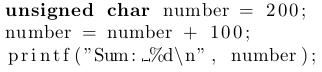
\includegraphics[scale=0.5]{mot2.png}
\end{frame}

\begin{frame}{Мотивация}
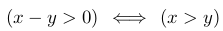
\includegraphics[scale=0.5]{mot1.png}\newline
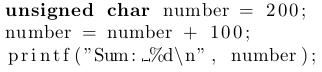
\includegraphics[scale=0.5]{mot2.png}\newline
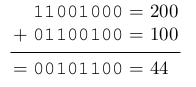
\includegraphics[scale=0.5]{mot3.png}
\end{frame}

\begin{frame}{Определения}
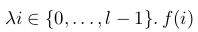
\includegraphics[scale=0.5]{lambda.png}\newline
\end{frame}

\begin{frame}{Определения}
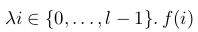
\includegraphics[scale=0.5]{lambda.png}\newline
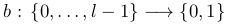
\includegraphics[scale=0.5]{vector.png}\newline
\end{frame}

\begin{frame}{Определения}
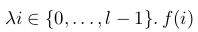
\includegraphics[scale=0.5]{lambda.png}\newline
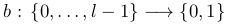
\includegraphics[scale=0.5]{vector.png}\newline
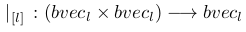
\includegraphics[scale=0.5]{or1.png}\newline
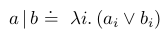
\includegraphics[scale=0.5]{or2.png}\newline
\end{frame}

\begin{frame}{Определения}
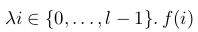
\includegraphics[scale=0.5]{lambda.png}\newline
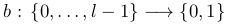
\includegraphics[scale=0.5]{vector.png}\newline
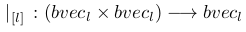
\includegraphics[scale=0.5]{or1.png}\newline
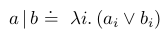
\includegraphics[scale=0.5]{or2.png}\newline
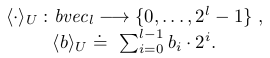
\includegraphics[scale=0.5]{unsigned.png}\newline
\end{frame}

\begin{frame}{Определения}
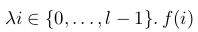
\includegraphics[scale=0.5]{lambda.png}\newline
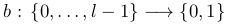
\includegraphics[scale=0.5]{vector.png}\newline
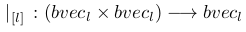
\includegraphics[scale=0.5]{or1.png}\newline
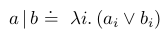
\includegraphics[scale=0.5]{or2.png}\newline
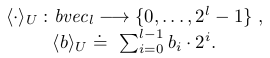
\includegraphics[scale=0.5]{unsigned.png}\newline
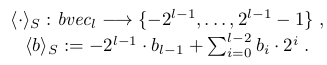
\includegraphics[scale=0.5]{signed.png}\newline
\end{frame}

\begin{frame}{Определения}
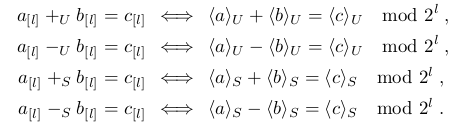
\includegraphics[scale=0.5]{sum.png}\newline
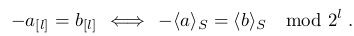
\includegraphics[scale=0.5]{unary.png}\newline
\end{frame}

\begin{frame}{Определения}
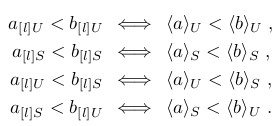
\includegraphics[scale=0.5]{rel.png}\newline
\end{frame}

\begin{frame}{Определения}
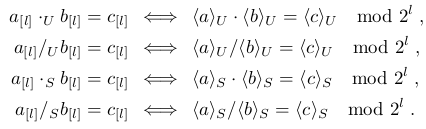
\includegraphics[scale=0.5]{mul.png}\newline
\end{frame}

\begin{frame}{Определения}
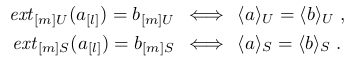
\includegraphics[scale=0.5]{ext.png}\newline
\end{frame}

\begin{frame}{Определения}
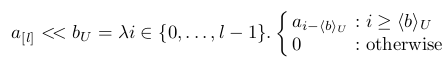
\includegraphics[scale=0.5]{sh0.png}\newline
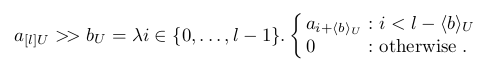
\includegraphics[scale=0.5]{sh1.png}\newline
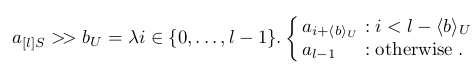
\includegraphics[scale=0.5]{sh2.png}\newline
\end{frame}

\begin{frame}{Алгоритм}
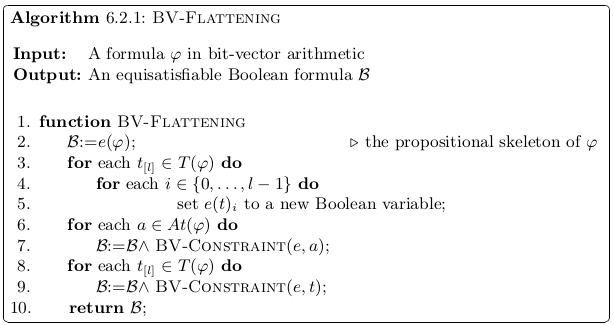
\includegraphics[scale=0.5]{algo.png}\newline
\end{frame}

\begin{frame}{Замены}
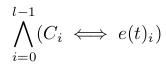
\includegraphics[scale=0.5]{skel.png}\newline
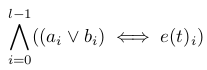
\includegraphics[scale=0.5]{or3.png}\newline
\end{frame}

\begin{frame}{Замены}
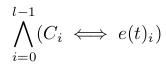
\includegraphics[scale=0.5]{skel.png}\newline
\end{frame}

\begin{frame}{Замены}
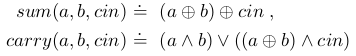
\includegraphics[scale=0.5]{sum1.png}\newline
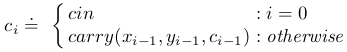
\includegraphics[scale=0.5]{sum2.png}\newline
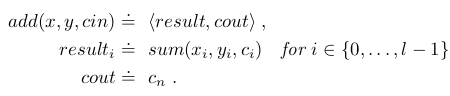
\includegraphics[scale=0.5]{sum3.png}\newline
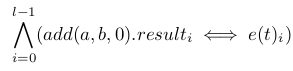
\includegraphics[scale=0.5]{sum4.png}\newline
\end{frame}

\begin{frame}{Замены}
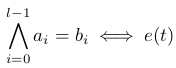
\includegraphics[scale=0.5]{rel1.png}\newline
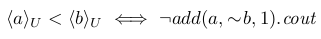
\includegraphics[scale=0.5]{rel2.png}\newline
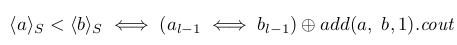
\includegraphics[scale=0.5]{rel3.png}\newline
\end{frame}

\begin{frame}{Замены}
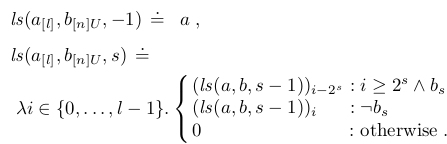
\includegraphics[scale=0.5]{ls.png}\newline
\end{frame}

\begin{frame}{Замены}
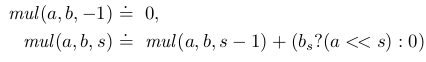
\includegraphics[scale=0.5]{mul1.png}\newline
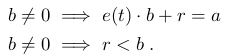
\includegraphics[scale=0.5]{div.png}\newline
\end{frame}

\begin{frame}
\includegraphics[scale=0.5]{../decision-procedure.png}
\end{frame}

\end{document}
